%!TEX root = ../main.tex
%%%%%%%%%%%%%%%%%%%%%%%%%%%%%%%%%%
% Links:
%
% Difficulty:
% Companies: 
%%%%%%%%%%%%%%%%%%%%%%%%%%%%%%%%%%

\chapter{Lowest Common Ancestor for BST}
\label{ch:lowest_common_ancestor}
\section*{Introduction}
The lowest common ancestor is an important concept in graph theory and it is
quite often a topic or a fundamental building block of coding interview questions.
Given a tree and two nodes $p$ and $q$, the lowest common ancestor  of $p$ and $q$, ($LCA(p,q)$) is defined as the lowest or deepest node that has both $p$ and $q$ as descendant.
In other words the LCA is the shared ancestor or $p$ and $q$ that is the farthest from the root of the tree.

In this chapter we will explore the problem of finding the LCA for a tree of a particular kind: binary search. This constraint simplify the general problem of finding LCA greatly. 
\section{Problem statement}
\begin{exercise}
	Write a function that takes a binary search tree $T$, and two nodes $p$ and $q$ and returns their lowest common ancestor.

	\begin{example}
		\hfill \\
		Given the tree in Figure \ref{fig:lowest_common_ancestor:example1} the lowest common ancestor for nodes:
		\begin{itemize}
			\item $p = 2$, $q=12$ is node $3$
			\item $p = 12$, $q=3$ is node $12$
			\item $p = 18$, $q=1$ is the root node $13$
		\end{itemize}
		\label{ex:lower_common_ancestor:example1}
	\end{example}
\end{exercise}

\begin{figure}
	\centering
	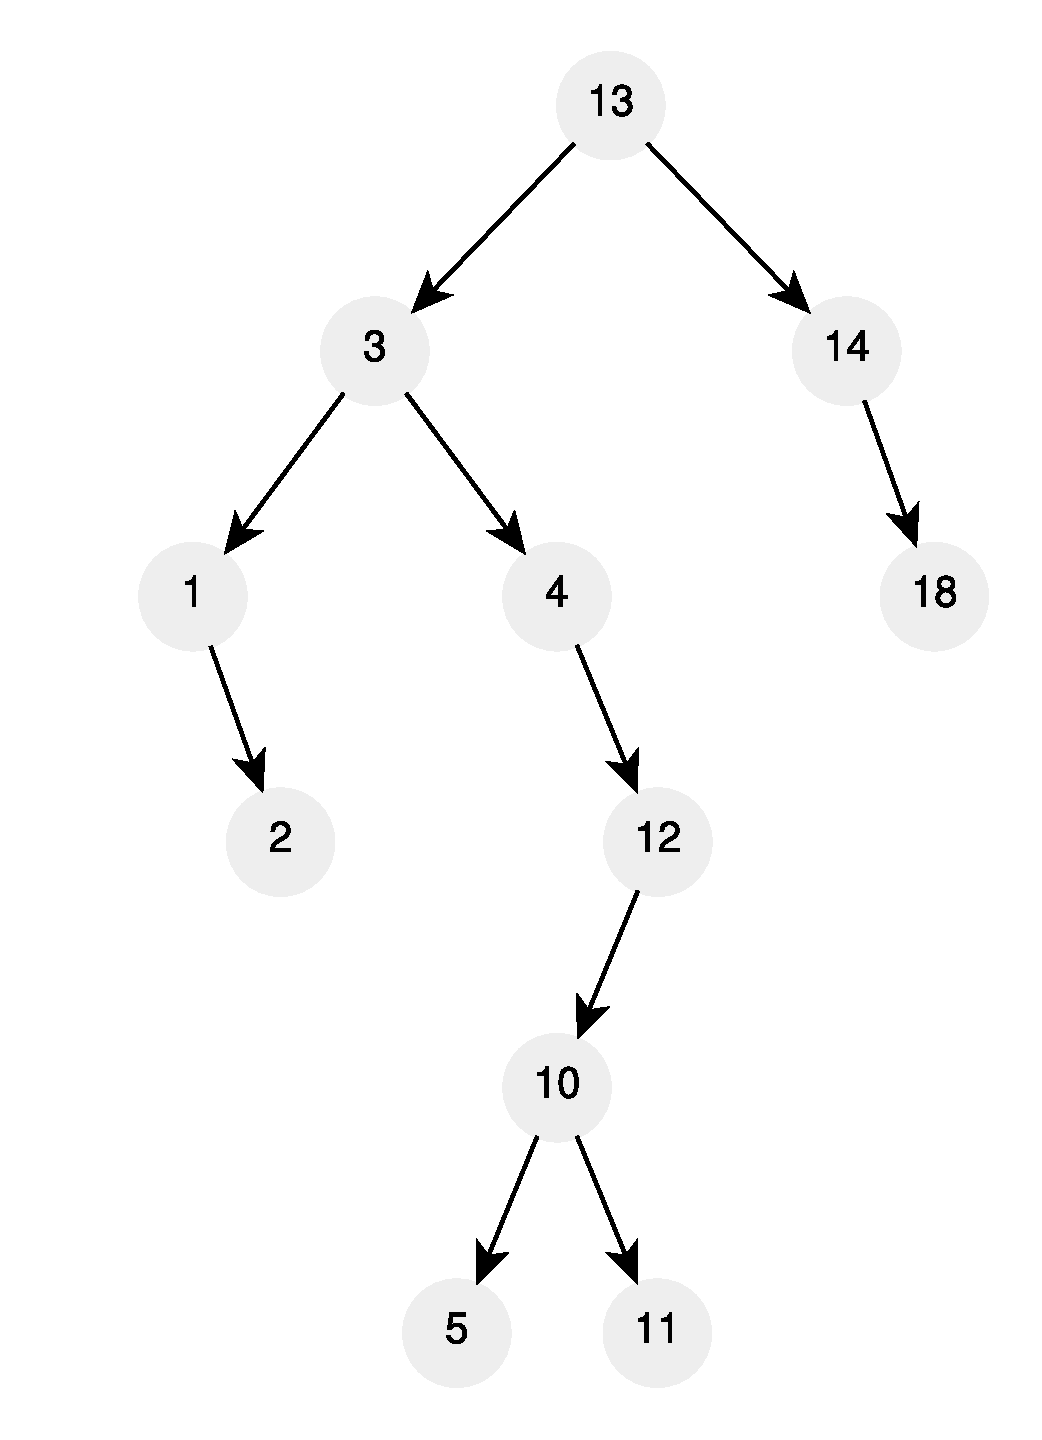
\includegraphics[width=0.4\textwidth]{sources/lowest_common_ancestor/images/example1}
	\caption[Sample short cpation]{Binary Search tree of Example \ref{ex:lower_common_ancestor:example1}}.
	\label{fig:lowest_common_ancestor:example1}
\end{figure}

\section{Clarification Questions}

\begin{QandA}
	\item 
	\begin{answered}
		\textit{}
	\end{answered}
	
\end{QandA}

\section{Discussion}
\label{lowest_common_ancestor:sec:discussion}


\subsection{Brute-force}
\label{lowest_common_ancestor:sec:bruteforce}

\begin{minipage}{\linewidth}
	\lstinputlisting[language=c++, caption={Sample Caption},label=list:lowest_common_ancestor]{sources/lowest_common_ancestor/lowest_common_ancestor_solution1.cpp}
\end{minipage}
